\documentclass[runningheads]{llncs}

\usepackage[utf8]{inputenc}
\usepackage[T1]{fontenc}
\usepackage{graphicx}
\usepackage{mathtools}
\usepackage{amssymb}
\usepackage{amsmath}
\usepackage{amsfonts}
\usepackage{hyperref}
\usepackage{bbm}
\usepackage{newunicodechar}
\usepackage{minted}
\usepackage{xcolor}
\usepackage{tikz}



\newcommand{\inl}[1]{\mintinline[breaklines, breakafter=→, escapeinside=||]{java}{#1}}
\newcommand{\classheader}{\text{class C<} \overline{\text{X}} \vartriangleleft \overline{\text{N}} \text{>} \vartriangleleft \text{N}}
\newcommand{\xn}{\text{<} \overline{\text{X}} \vartriangleleft \overline{\text{N}} \text{>}}
\newcommand{\yp}{\text{<} \overline{\text{Y}} \vartriangleleft \overline{\text{P}} \text{>}}
\newcommand{\ot}[1]{\overline{\text{#1}}}
\newcommand{\vv}[1]{\text{<} #1 \text{>}}
\newcommand{\txn}[3]{\text{[#1/#2]#3}}
\newcommand{\tsxsn}[3]{\text{[}\ot{#1}/\ot{#2}\text{]#3}}
\newcommand{\tsxsns}[3]{\text{[}\ot{#1}/\ot{#2}\text{]}\ot{#3}}
\newcommand{\tsxsnd}[5]{\text{[}\ot{#1}/\ot{#2}\text{]}\text{[}\ot{#3}/\ot{#4}\text{]#5}}
\newcommand{\tsxsnsd}[5]{\text{[}\ot{#1}/\ot{#2}\text{]}\text{[}\ot{#3}/\ot{#4}\text{]}\ot{#5}}
\newcommand{\cm}{\text{C} \xn \text{.m}}
\newcommand{\oto}[1]{\overline{#1} \to #1}
\newcommand{\sprod}[1]{\raisebox{.5ex}{\scalebox{#1}{$\prod$}}}
\newcommand{\mtype}{\text{mtype} ( \text{m}, \ \text{N}, \ \sprod{0.7} )}
\newcommand{\mtypeC}[1]{\text{mtype} ( \text{m}, \ #1, \ \sprod{0.7} )}
\newcommand{\fresh}[1]{#1 \ \text{fresh}}
\newcommand{\texpr}[1]{\text{TYPEExpr}((\sprod{0.7}; \overline{\eta}), #1)}
\newcommand{\nvt}[2]{\text{#1<}\ot{#2}\text{>}}
\newcommand{\class}[2]{\classheader \ \{ \ \ot{#1} \ \ot{#2} ; \ [\text{K}] \ \ot{M} \ \} }
\newcommand{\cand}{\text{C} \cup}
\newcommand{\cxnm}[4]{\text{#1} \text{<} \text{#2} \vartriangleleft \text{#3} \text{>}. \text{#4}}
\newcommand{\nvtt}[2]{\text{#1} \text{<} #2 \text{>}}
\newcommand{\fa}[1]{\text{a}_{#1}}
\newcommand{\xa}[2]{\text{#1}_{#2}}
\newcommand{\pink}[1]{\textcolor{purple}{#1}}
\newcommand{\blue}[1]{\textcolor{blue}{#1}}
\newcommand{\green}[1]{\textcolor{teal}{#1}}
\newcommand{\black}[1]{\textcolor{black}{#1}}


\makeatother

\title{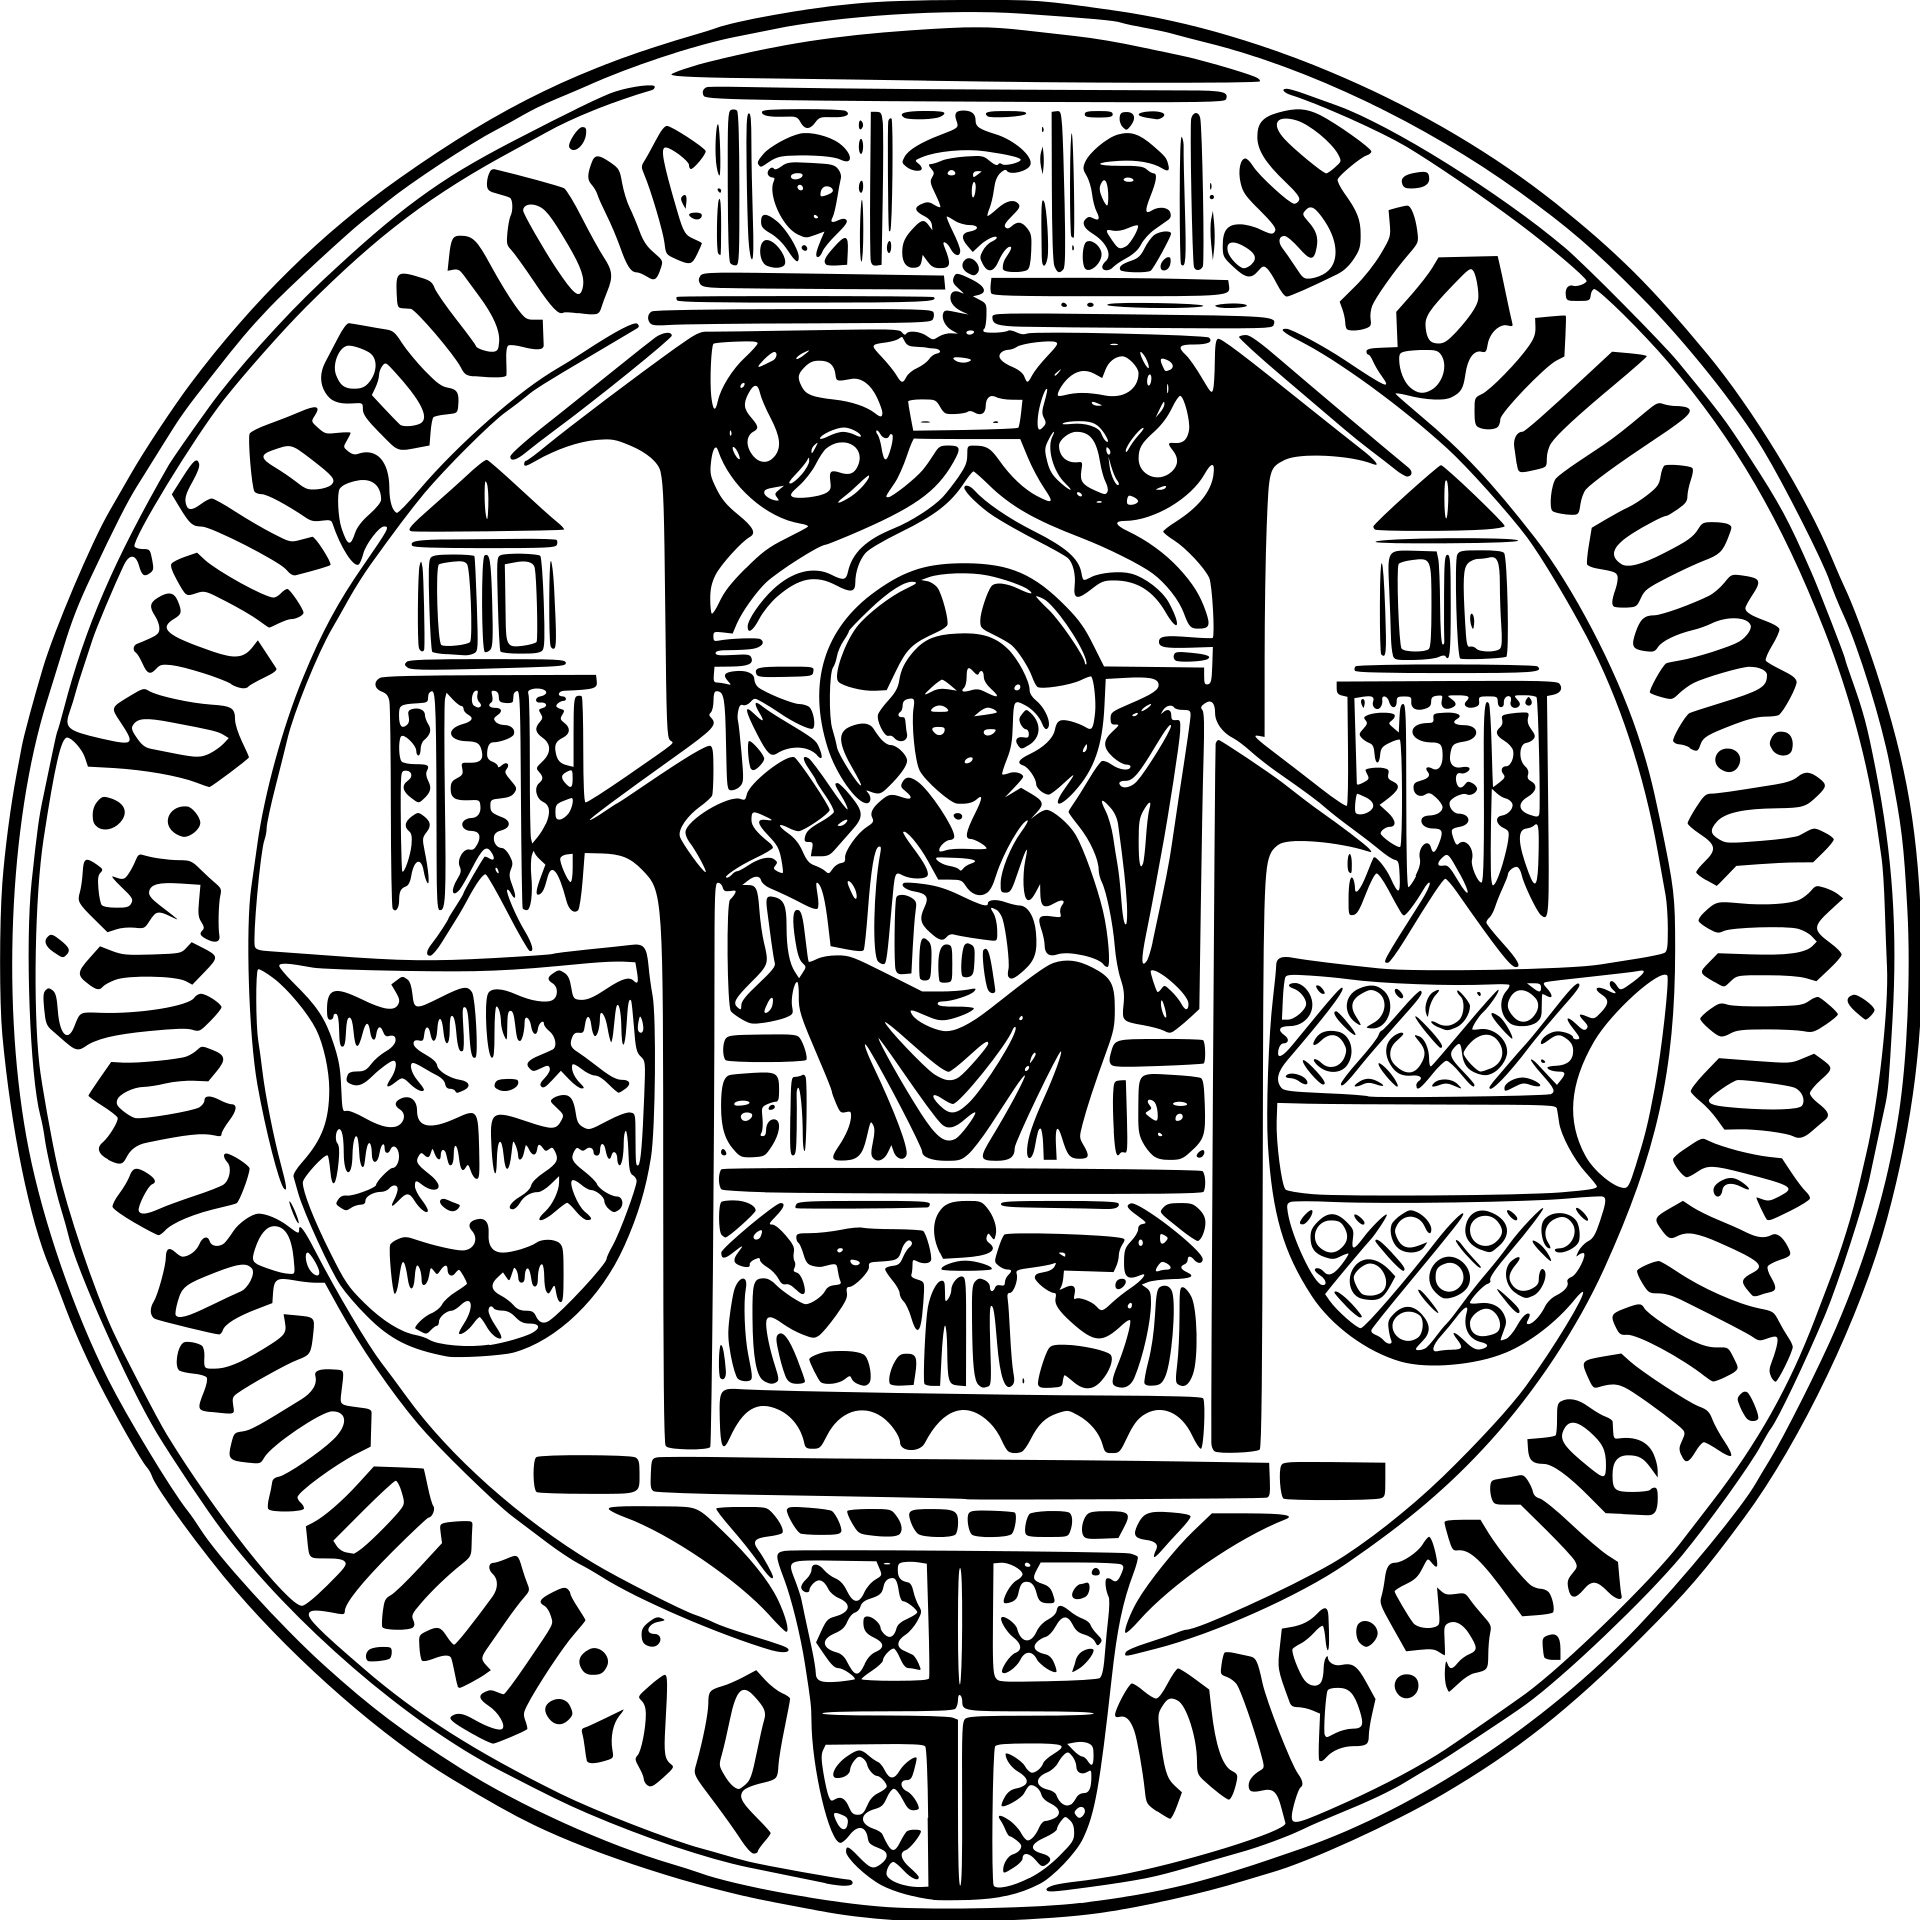
\includegraphics[width=0.29\textwidth]{logo.png}~
\\[1cm]
An Implementation of Type Inference for Featherweight Generic Java}
\titlerunning{Implementation of Type Inference for Featherweight Generic Java}
\institute{Chair of Programming Languages, University of Freiburg \\ \email{timpe.hoerig@students.uni-freiburg.de}}
\author{Timpe Hörig}


\begin{document}

\let\oldaddcontentsline\addcontentsline
\def\addcontentsline#1#2#3{}
\maketitle
\def\addcontentsline#1#2#3{\oldaddcontentsline{#1}{#2}{#3}}


\noindent\makebox[\linewidth]{\bf{Bachelor Thesis}}
\\

\noindent\makebox[\linewidth]{Examiner: Prof. Dr. Peter Thiemann}
\noindent\makebox[\linewidth]{Advisor: Prof. Dr. Peter Thiemann}

\begin{abstract}
  Type systems are an essential and powerful part of every modern programming language.
However, to be forced to explicitly specify every type signature can be tiring.
Type inference algorithms relieve the programmer from the burden to write type signatures themselves.
My work describes and implements a global type inference algorithm for Featherweight Generic Java: a minimal core calculus for Java with support for generics.
The type inference algorithm is able to infer all method types for a program with specified class headers and field types.
Originally, the inference algorithm was developed by Andreas Stadelmeier, Martin Plümicke and Peter Thiemann in the paper: "Global Type Inference for Featherweight Generic Java".

\end{abstract}
\begin{abstract}\textbf{(german)}
  Typsysteme sind ein wichtiger und mächtiger Bestandteil einer jeden mordernen Programmiersprache.
Jede Typsignatur explizit angeben zu müssen kann nicht nur nervig sein, auch den generellsten Typen zu finden kann manchmal schwierig sein.
Wenn das Typsystem die Typesignatur selbst herleiten kann, entstehen diese Probleme erst gar nicht.
Das ist ein globaler typinferenz Algorhythmus für Featherweight Generic Java ein minimales Modell von Java (Featherweight Java) erweitert mit generischen Typen.
Hier wird der type inferenz Algorhythmus implementiert wie er in dem Paper "Global Type Inference for Featherweight Generic Java" von Andreas Stadelmeier, Marting Plümicke und Peter Thiemann beschrieben ist.

\end{abstract}

\setcounter{tocdepth}{2}
\tableofcontents
\newpage

\section{Introduction}
\subsection{Type Systems}
Consider the following definition of the function \verb|increment| which takes an argument \verb|N|,
increments it by one and returns the result.
\begin{minted}[escapeinside=||]{java}
  |\black{increment}|(n) {
    |\pink{return}| n + 1;
  }
\end{minted}
Calling this function with an \verb|Integer|, for example 1, returns 2.
However, calling it with a \verb|String| results in a type error, because addition between a \verb|String|
and an \verb|Integer| is not defined.
Errors such as that are easy to make but cause the program to crash at runtime.
With type systems it is possible to detect such errors at compile time and thus increases the quality of programs dramatically.
In order to detect such errors at compile time, additional information is given to the function declaration.
Consider the previous example but now with type annotations.
\begin{minted}[escapeinside=||]{java}
  |\green{Integer} \black{increment}|(|\green{Integer}| n) {
    |\pink{return}| n + 1;
  }
\end{minted}
Writing the type \verb|Integer| in front of the function name indicates the function's return type.
The arguments are annotated by writing their types in front of each argument.
Now the type system knows of which type the argument must be and thus calling \verb|increment| with a \verb|String| results in a type error at compile time rather than at runtime.

\subsection{Type Inference}
In order to correctly typecheck a whole program, everything that has a type needs an explicit type annotated.
Even if the type annotation seems to be redundant, for example, for an instantiation of a variable.
Another downside might be, that programmers do not always annotate the most general type. Consider the function \verb|_+_| without any type annotations. This function works for all types that support the addition operator for instance \verb|Int|, \verb|Double| or \verb|Float|.
Annotating the function \verb|_+_| with one of those types would mean it is not possible to call it with another one.\\
So having the advantages of a type system without being forced to write the additional information yourself would be optimal. Type inference does just this.
However, type inference has its boundaries. Inferring every type without any information is often not just hard but impossible. Different languages have different restrictions to make global type inference possible.

\subsection{Featherweight Generic Java}
Java is one of the most popular programming languages world wide. Extending Java with new features and providing proofs of soundness becomes more and more difficult as Java becomes more and more complex.
To be able to provide proofs about complex programming languages often a smaller version of them is defined that contains less features but behaves similarly.
Extending those smaller versions with new features leads to languages still small enough so providing proofs not only becomes feasible but handy.
Featherweight Java is exactly that. A smaller version of Java. In fact, it is so small that almost all features are dropped, even assignments. Due to that Featherweight Java a functional subset of Java.
Featherweight Java only contains classes with fields, methods and inheritance as well as five different forms of expressions: variables, field lookups, method invocations, object creation and castings.
As Java itself is not a functional programming languages it is easy to see that Featherweight Java is not as expressive as Java. But due to its similar behaviour it is still possible to draw back conclusions to the full Java.

A typical Featherweight Java program may look like this:

\begin{minted}[escapeinside=||]{java}
  |\pink{class} \green{Pair} \pink{extends} \green{Object}|{
    |\green{Object} fst|;
    |\green{Object} snd|;

    |\green{Pair} \black{setfst}|(|\green{Object}| newfst) {
      |\pink{return new} \green{Pair}|(|newfst, this.snd|);
    }
  }

  (|\pink{new} \green{Pair}|(
    |\pink{new} \green{Pair}|(|\pink{new} \green{Object}|(), |\pink{new} \green{Object}|()),
    |\pink{new} \green{Object}|()
  ).|fst|).|fst|
\end{minted}

A Featherweight Java program always consists of two parts. Firstly, one or more class definitions and secondly, an expression to be evaluated.

As well as Java, Featherweight Java includes a type system. With the type annotations given in the class definitions Featherweight Java is able to typecheck the given expression.
In the example above the most inner expression that has a fixed type is the object creation of \verb|new Pair(new Pair(new Object(),| \verb|new Object()),| \verb|new Object())|. It has type \verb|Pair|.
Then, the field \verb|fst| is accessed. Because the field \verb|fst| of class \verb|Pair| is annotated with \verb|Object|, the resulting type is \verb|Object|. Even if the expression itself is \verb|new Pair(new Object(),| \verb|new Object())|.
Now, trying to access the field \verb|fst| for the second time is not possible. Even in case the expression of the field lookup is an object creation of \verb|Pair|, the type of the expression is \verb|Object|. Consequently, it results in a compile time error.

This problem can be solved by giving fields a type parameter \verb|X| instead of a concrete type like \verb|Object|.
Extending Featherweight Java with generics leads to Featherweight Generic Java.
Type parameters are just like normal parameters but they range over types. In Featherweight Generic Java every type parameter is given an upper bound.
In the following example the type parameters \verb|X| and \verb|Y| are both introduced with the upper bound \verb|Object|.
That means both type parameters can range over any types that are a subtype of \verb|Object|.

Type parameters can also be used in method declarations to set relations between different arguments and or the return type.
When a class is instantiated the type parameters are instantiated with a concrete type.

Rewriting the previous example results in:

\begin{minted}[escapeinside=||]{java}
  |\pink{class} \green{Pair}|<|\green{X} \pink{extends} \green{Object}|<>,
             |\green{Y} \pink{extends} \green{Object}|<>> |\pink{extends} \green{Object}|<>{
    |\green{X} fst|;
    |\green{Y} snd|;

    <|\green{Z} \pink{extends} \green{Object}|<>> |\green{Pair}|<|\green{Z}|, |\green{Y}|> |setfst|(|\green{Z} newfst|) {
      |\pink{return new} \green{Pair}|(newfst, |this.snd|);
    }
  }

  (|\pink{new} \green{Pair}|<|\green{Pair}|<|\green{Object}|<>, |\green{Object}|<>>, |\green{Object}|<>>(
    |\pink{new} \green{Pair}|<|\green{Object}|<>, |\green{Object}|<>>(|\pink{new} \green{Object}|<>(), |\pink{new} \green{Object}|<>()),
    |\pink{new} \green{Object}|<>()
  ).|fst|).|fst|
\end{minted}

Now, trying to access the field \verb|fst| results in the same expression but with type \verb|Pair<Object<>, Object<>>|. That is why the second field lookup is successful.

Generics are very powerful and useful to have but at the same time make type annotations much more complicated and longer.
Adding type inference to Featherweight Generic Java would make it possible to rewrite the example above as follows:

\begin{minted}[escapeinside=||]{java}
  |\pink{class} \green{Pair}|<|\green{X} \pink{extends} \green{Object}|<>,
             |\green{Y} \pink{extends} \green{Object}|<>> |\pink{extends} \green{Object}|<>{
    |\green{X} fst|;
    |\green{Y} snd|;

    |setfst|(newfst) {
      |\pink{return new} \green{Pair}|(newfst, |this.snd|);
    }
  }

  (|\pink{new} \green{Pair}|(|\pink{new} \green{Pair}|(|\pink{new} \green{Object}|(), |\pink{new} \green{Object}|()),
            |\pink{new} \green{Object}|()).|fst|).|fst|
\end{minted}

Here, almost every type annotation is dropped except for class headers and field types.
\\
\\
The following sections first describe Featherweight Generic Java and Global Type Inference formally as it is described in the paper "Global Type Inference for Featherweight Generic Java"\cite{FGJ} by Stadelmeier et al. Afterwards, it is shown how the Global Type Inference Algorithm is implemented. There are a few changes to bring the formalisation closer to the implementation.


\section{Featherweight Generic Java}
\begin{figure}
    \begin{align*}
        \text{T} &:= \text{X} \ | \ \text{N}\\
        \\
        \text{N} &:= \text{C} \vv{\ot{T}}\\
        \\
        \text{L} &:= \text{class} \ \text{C} \xn \ \vartriangleleft \ \text{D} \{ \ \ot{T} \ \ot{f} \ [\text{K}] \ \ot{M} \ \}\\
        \\
        \text{M} &:= \text{m}(\ot{x}) \ \{\text{return e}\}\\
        \\
        \text{e} &:= \text{x} \ | \ \text{e.f} \ | \ \text{e.m(}\ot{e}\text{)} \ | \ \text{new C(}\ot{e}\text{)} \ | \ \text{(C)e}
    \end{align*}
    \caption{Syntax}
    \label{syntax}
\end{figure}

Figure \ref{syntax} defines the syntax of Featherweight Generic Java. Types (\inl{T} and \inl{N}), class definitions (\inl{L}), method definitions (\inl{M}) and expressions (\inl{e}).

\subsection{Types}

There are two different kinds of types (\inl{T}, \inl{U}, \inl{V}) in Featherweight Generic Java.
Type parameters (\inl{X}, \inl{Y}, \inl{Z}) and types other than type parameters (\inl{N}, \inl{P}, \inl{Q}).
Writing $\ot{T}$ short for $\text{T}_1, \text{T}_2, ... \text{T}_n$.

\subsection{Class Definitions}

A class definition \inl{L} always begins with the keyword \inl{class} followed by its name. Then every type parameter and its upper bound that are used as a field type in the class definition are declared within \inl{<>} writing $\vartriangleleft$ as shortcut for the keyword \inl{extends}.
Followed by the name of the superclass. In the body of a class definition the fields (\inl{f}, \inl{g}) of the class are defined, writing their types infront of them. Followed by the optional constructor \inl{K} and all method definitions $\ot{M}$.

\subsection{Method Definition}

As this is a type inference algorithm every type annotations of methods can be dropped. Leading a method definition only to consist of its name \inl{m}, its arguments $\ot{x}$ and a single expression \inl{e} which is returned.

\subsection{Expressions}

An expression \inl{e} can be in five different forms. First, a simple variable \inl{x}. Second, a field lookup written \inl{e.f}. Third, a method invocation that takes one expression for each argument. Fourth, an object creation indicated by the keyword \inl{new} followed by the name of the new Object and its arguments. Fifth, a cast.
A cast binds less than any other expression. Method calls and object creation do not need any instantiation of their generic type annotations.

\subsection{Type Annotation}

Every type annotation except for field types and their upper bounds in class definitions can be dropped.

\subsection{Constructor}

\begin{align*}
    \text{K} &:= \text{C}(\ot{f}, \ \ot{g}) \ \{ \text{super}(\ot{g}); \ \text{this}.\ot{f}=\ot{f}; \}
\end{align*}

In Featherweight Java as well as in Featherweight Generic Java a constructor is always required. The constructor has always the same form.
The name of the constructor is always the name of the class itself. For every field of the class the constructor takes exactly one argument which must have the same name as the field it belongs to.
The body of the constructor always consists of two parts. First, a call to super, in which all arguments with field names defined in superclasses are passed on.
Second, every other argument is initialized in the form \inl{this.f=f}.

As a constructor does not contain any information that cannot be found somewhere else in the class definition, writing the constructor for every class definition is redundant and can be dropped in this implementation.


\section{Auxiliary Functions}
In the following sections all auxiliary functions that are used in the typeinference algorithm are specified.

\subsection{Substitution}

\begin{align*}
1&: \txn{T}{X}{N}
\\
\\
2&: \tsxsn{T}{X}{N}
\\
\\
3&: \tsxsns{T}{X}{N}
\end{align*}

The first rule (1) shows the standart substitution rule. In a non variable type N every variable type X is replaced by the given type T.
\\
The second rule (2) is short for \inl{[T_1/X_1, ... , T_n/X_n]N}.
\\
The third rule (3) is short for \inl{[T_1/X_1, ... , T_n/X_n]N_1, ... , [T_1/X_1, ... , T_n/X_n]N_n}.
\\
These rules are implemented in different functions using pattern matching on the different type types.

\subsection{Substitution on constraints}

\begin{align*}
    1:& \quad \txn{T}{a}{C}\\
    \\
    2:& \quad \txn{a}{b}{C}
\end{align*}

Substitution is also possible on constraint sets. Type variables can be replaced by types (1) or by other type variables (2).

\subsection{Subtyping}

\begin{figure}[H]
    \begin{align*}
1&: \ \Delta \vdash \text{T} <: \text{T}
\\
\\
2&: \ \frac{\Delta \vdash \text{S} <: \text{T} \quad \Delta \vdash \text{T} <: \text{U}}{\Delta \vdash \text{S} <: \text{U}}
\\
\\
3&: \ \Delta \vdash \text{X} <: \Delta(\text{X})
\\
\\
4&: \ \frac{
    \begin{matrix}
        \classheader \ \{...\} \\
        \Delta \vdash \ot{T} ok \quad \Delta \vdash \ot{T} <: \tsxsns{T}{X}{N}
    \end{matrix}}
    {\Delta C<\ot{T}> \ ok}
    \end{align*}
    \caption{Subtyping}
    \label{subtyping}
\end{figure}

By definition a type is always a subtype of itself. Subtyping is also transitive and the environment delta $\Delta$ maps every type variable to its upper bound.

\subsection{Field Lookup}

\begin{align*}
    \text{fields}(\text{Object}) = \{\}\\
    \\
    \frac{\class{S}{f} \quad \text{fields}(\tsxsn{T}{X}{N}) = \ot{U} \ \ot{g} }{\text{fields}(\nvt{C}{T}) = \ot{U} \ \ot{g}, \ \tsxsns{T}{X}{S} \ \ot{f}}\\
\end{align*}

A field lookup on a class \inl{C} returns every field of \inl{C} with its type and also every field with its type for all superclasses of \inl{C}. \inl{Object} itself has no fields thus \inl{fields(Object)} returns the empty dictionary.
The type variables need a special treatment here. The field types of a class \inl{C} may include type variables, these must be substituted with the types the class is instantiated with. This also needs to be done for the superclass of \inl{C}.

\subsection{Method Type Lookup}

In Featherweight Generic Java methods of superclasses are inherited. Hence method type lookups on classes with or without the method defined can be possible. If the method is defined in the class, the method type signature can be read of the method type environment. Once again generic type variables may occur in that type signature and must be substituted.
If the method is not defined in the class \inl{C}, then \inl{mtype} is called on the superclass of \inl{C} where generic type variables are substituted by the types the class \inl{C} is instantiated with.

\subsection{Generic Supertype}

\begin{align*}
    \text{genericSupertype} (\text(C), \ot{T}, \text{C} ) = \ot{T}\\
    \\
    \frac{ \text{class} \ \text{C} \yp \vartriangleleft \nvt{C'}{M} \ \{ ... \} }{ \text{genericSupertype} ( \text{C}, \ot{T}, \text{D} ) = \text{genericSupertype} ( \text{C'}, \tsxsns{T}{Y}{M}, \text{D} ) }\\
\end{align*}

GenericSupertype takes two subtype related classes C and D and a list of types $\ot{T}$ as arguments. If the two classes are the same, then the list of types $\ot{T}$ is returned. Otherwise the function is recursively called with the superclass C' of C.
However, the superclass C' may have different generic type variables than C. That is why $\ot{T}$ is replaced by $\ot{M}$ where $\ot{M}$ are the generic type variables of C', but the generic type variables $\ot{Y}$ may occur in $\ot{M}$, thus $\ot{T}$ is substituted for $\ot{Y}$ in $\ot{M}$.


\section{Type Inference}
The type inference algorithm looks at one class after another. Therefore all classes must be ordered in a way that method calls only call methods from classes defined before the current class.
However, this does not constrain the algorithm as a program where this is not the case can be transformed to a program where it is.
This transformation is shown in the paper [...].
\\
In the following it is assumed that a program always fulfills this condition.

The algorithm mainly consist of two parts:
First, constraint generation and second, constraint solving.
As solving the constraints can lead to multiple solutions for a single class, simply one solution is assumed. If the algorithm later fails, it backtracks and assumes the next solution.

\begin{figure}[H]
    \begin{align*}
        \text{FJTypeInference}&(\prod, \ \classheader \{ ... \}) = \\
        \text{let} (\overline{\lambda}, \ \text{C}) &= \text{FJType}(\prod, \classheader \{ ... \}) \\
        (\sigma, \yp) &= \text{Unify}(\text{C}, \overline{\text{X}} <: \overline{\text{N}}) \\
        \text{in} \prod \cup \ \{( & \cm \ : \ \yp \ \oto{\sigma(a)}) \ | \ (\cm : \oto{a} ) \in \overline{\lambda} \}
    \end{align*}
    \caption{Type Inference}
    \label{type_inference}
\end{figure}


\section{FJType}
\inl{FJType} is the function that generates constraints for a class. It takes the definition of that class and the method type environment where all the method signatures that have already been inferred from earlier classes are in.
It returns a tuple consisting of a set of method signatures 'lambda' with new type variables and a constraint set C which constraints those type variables.

In Featherweight Generic Java methods can be overridden with covariant types. If a method is overridden or not can be checked by calling \inl{mtype} on the class's supertype.
If it does not find a method signature the type signature can be initialized with some new type variables which have only the constraint to be subtypes of \inl{Object}.
However, if the \inl{mtype} lookup is successful the constraints look different. The return type of the current method needs to be a subtype of the return type of the overridden method.
Whereas the types of the arguments stay the same. Then the method signature is added to the global method type environment.
This is done for every method definition of the class. Then the \inl{MethodType} function is called on every method defined in the class. Therefore, every method has access to the full method type environment.
The method type environment and the generated constraints together with the constraints generated by \inl{MethodType} are returned.

\begin{figure}[H]
    \begin{align*}
        \text{FJType}(\prod, \classheader \{ \ot{T} \ \ot{f}; \ \ot{M} \}) = \\
        \text{let} \ \overline{a}_m \ \text{be fresh type variables for each m} \in \ot{M} \\
        \overline{\lambda}_0 = \{\cm : \ \yp \ot{T} \to a_m \ | \ \text{m} \in \ot{M}, \ \mtype = \yp \ot{T} \to \text{T} \}\\
        C_0 = \{ a_m < \text{T} \ | \ \text{m} \in \ot{M}, \ \mtype = \yp \oto{T} \}\\
        \overline{\lambda}' = \{ ( \cm : \ \overline{a} \to a_m ) \ | \ \text{m} \in \ot{M}, \ \mtype \ \text{not \ defined}, \fresh{\overline{a}} \}\\
        C_m = \{\{ a_m < \text{Object}, \overline{a} < \ot{Object} \} \ | \ ( \cm : \ \overline{a} \ to a_m) \in \overline{\lambda}' \} \\
        \prod = \prod \cup \overline{\lambda}' \cup \overline{\lambda}_0\\
        \text{in} \ (\prod, C_0 \cup C_m \cup \cup{text{m} \in \ot{m}} \text{TYPEMethod}(\prod, C \vv{\ot{X}}, \text{m}))
    \end{align*}
    \caption{FJType}
    \label{fjtype}
\end{figure}

\subsection{Method Type}

\inl{MethodType} takes the method type environment, the class header \inl{C<\overline{X}>} of the class that is currently checked and the method definitions as arguments.
It first brings the type signature of the current method in scope and then calls \inl{TypeExpression} on the expression \inl{e} inside the body of the method. In this call also a type environment for variables is created, where \inl{this} has the type C<X'> and the arguments of the method are read from the type signature brought into the scope earlier.
\inl{TypeExpression} returns a tuple of the type \inl{R} of \inl{e} and the generated constraints. The generated constraints together with the constraint that \inl{R} must be a subtype of the return type of the method signature is returned.

\subsection{Type Expressions}
The last function for generating constraints is \inl{Type Expression}. It takes the method type environment, the variable type environment created by \inl{Type Method} and an expression \inl{e} as arguments.
The expression \inl{e} is matched against the five possible forms for an expression and is handled differently for each.

\subsection{Variable}
If the expression is a simple variable it's type is looked up in the variable type environment and together with an empty set is returned. The empty set is returned because a simple variable does not generate any constraints.

\subsection{Field Lookup}
In case of a field lookup \inl{e.f} first the \inl{Type Expression} function recursively is called on the expression \inl{e}, returning a
type R and a constraint set $C_R$. Now the difficult part is to find out which class the field \inl{f} belongs to. The solution is simple,
just generate a constraint set for every class \inl{C} that has the field \inl{f} and put them together in one big or-constraint.
The constraint set for one class consists of three constraints. One that constraints the returned type R to be a subtype
of the class \inl{C} where the type variables of \inl{C} are replaced by some fresh type variables \inl{\overline{a}}. One that constraints the resulting type of the field lookup
to be equal to the type of the corresponding field in \inl{C}. And another one that constraints every $a_i$ of \inl{\overline{a}} to be a subtype of the bounding type of the corresponding type variable it replaces.

\subsection{Method Invocation}
A method invocation imposes the same problem that a field lookup did and therefore is solved in a similar way. But first for the
expression the method \inl{m} is invoked on and every expression that is passed as an argument to \inl{m} \inl{Type Expression}
recursively is called on. Then for every method signature of a method with name \inl{m} in the method type environment an constraint set is generated.


\section{Unify}
The function \verb|Unify| solves a constraint set. Solving the constraints may lead to no, one or multiple possible solutions. If there is more than one solution, simply the first solution is chosen. If there is no solution, the overall algorithm backtracks to the last class where there was more than one solution and assumes the next one. Then, it starts again from there.
A solution is found, if the constraint set can be transformed into solved form. A constraint set is in solved from, if it only contains constraints of the following four forms:

\begin{align*}
    1.& \quad \text{a} < \text{b}\\
    \\
    2.& \quad \text{a} = \text{b}\\
    \\
    3.& \quad \text{a} < \text{C<} \ot{T} \text{>}\\
    \\
    4.& \quad \text{a} = \text{C<} \ot{T} \text{>} \ \text{with a} \notin \ot{T}\\
    \\
    \text{No variable is allowed to occur } & \text{twice on the left side of rules 3 and 4.}
\end{align*}

\verb|Unify| takes two arguments: First, the constraint set to solve. Second, a mapping from type parameters \verb|X| to their upper bound \verb|N|. This mapping represents the type parameters and their upper bounds of the current class that the overall algorithm is currently checking.
In order to circumvent a special treatment for these type parameters, all type parameters $X_i$ are treated as parameterless classes $X_i$<> with superclass $N_i$.
The constraint set $C$ given to \verb|Unify| may contain multiple or-constraints. Flattening them to constraint sets $C$' that only contain simple constraints leads to multiple $C$' that together cover all possible combinations of constraints.
The following steps are done for the first $C$'. If this leads to a solution, \verb|TypeInference| continues with the next class. Otherwise, the next $C$' is tried.

\subsubsection{Step 1}
The rules defined in Figure \ref{resolve_rules} are applied exhaustively to $C$'.

\begin{figure}[tp]
    \begin{align*}
        &\frac{\cand \{ \text{a} < \nvt{C}{T}, \ \text{a} < \nvt{D}{V} \} }{ \cand \{ a < \nvt{C}{T}, \ \nvt{C}{T} < \nvt{D}{V} \} } \quad \Delta \vdash \nvt{C}{X} <: \nvt{D}{N} &\text{match}\\
        \\
        &\frac{\cand \{ \nvt{C}{T} < \text{a}, \ \nvt{D}{V} < \text{a} \} }{ \cand \nvt{C}{T} < \nvt{D}{V}, \ \nvt{D}{V} < \text{a} } \quad \Delta \vdash \nvt{C}{X} <: \nvt{D}{N} &\text{match reverse}\\
        \\
        &\frac{\cand \{ \text{a} < \nvt{C}{T}, \ \text{b} <^* \text{a}, \text{b} < \nvt{D}{U}  \} }{ \cand \{ \text{a} < \nvt{C}{T}, \ \text{b} <^* \text{a}, \ \text{b} < \nvt{D}{U}, \ \text{b} < \nvt{C}{T} \} } &\text{adopt}\\
        \\
        &\frac{\cand \{ \nvt{C}{T} < \text{a}, \ \text{a} <^* \text{b}, \nvt{D}{U} < \text{b} \} }{ \cand \{\nvt{C}{T} < \text{a}, \ \text{a} <^* \text{b}, \ \nvt{D}{U} < \text{b}, \ \nvt{C}{T} < \text{b} \} } &\text{reverse adopt}\\
        \\
        &\frac{\cand \{ \nvt{C}{T} < \nvt{D}{U} \} }{ \cand \{ \text{D<} \tsxsns{T}{X}{N} \text{>} = \nvt{D}{U} \} } \Delta \vdash \nvt{C}{X} <: \nvt{D}{N} &\text{adapt} \\
        \\
        &\frac{\cand \{ \nvt{D}{T} = \nvt{D}{U} \} }{\cand \{ \ot{T} = \ot{U} \} } &\text{reduce} \\
        \\
        &\frac{\cand \{ \text{a}_1 < \text{a}_2, \ \text{a}_2 < \text{a}_3, \ ..., \ \text{a}_n < \text{a}_1 \} }{\cand \{ \text{a}_1 = \text{a}_2, \ \text{a}_2 = \text{a}_3, \ ... \} } \quad \text{n} > 0 &\text{equals} \\
        \\
        &\frac{\cand \{ \text{a} = \text{a} \} }{\text{C}} &\text{erase} \\
        \\
        &\frac{\cand \{ \text{N} = \text{a} \} }{\cand \{ \text{a} = \text{N} \} } &\text{swap}
    \end{align*}
    \caption{resolve rules}
    \label{resolve_rules}
\end{figure}

For \verb|match| and \verb|adopt| the implementation also includes the dual rules.
Thus, only the highest non variable type can have an illegal upper bound by a type variable.
This decreases the amount of or-constraints generated.

\subsubsection{Step 2}
Check if one of the following cases applies. If not, the constraint set is in solved form:\\
1. $\{ \nvt{C}{T} < \nvt{D}{U} \}$ where \verb|C| cannot be a subtype of \verb|D|. As a result $C$' has no solution.\\
2. $\{ a < \nvt{C}{T}, \ a < \nvt{D}{U} \}$ where \verb|C| cannot be a subtype of \verb|D| and vice versa. Again, $C$' has no solution.\\
3. $\{ \nvt{C}{T} < a \}$\\
\\
In the last case the non variable type $\nvt{C}{T}$ has an upper bound. This upper bound is a type variable \verb|a| which is not allowed in Featherweight Generic Java.
This is solved by first searching the upper bound constraint of \verb|a|. If no such constraint exists, \verb|Object| is chosen as the upper bound. Then, for every possible class
from $\nvt{C}{T}$ up to the upper bound an or-constraint is generated which then replaces the one or two constraints it was generated from.
The or-constraint is generated as follows:

\begin{align*}
    \text{expandLB} ( \nvt{C}{T} < a, \ a < \nvt{D}{U} ) = \{ \{ &a = \tsxsn{T}{X}{N} \} \\
     &| \ \Delta \vdash \nvt{C}{X} < \text{N}, \ \Delta \vdash \text{N} < \nvt{D}{P} \}\\
    \text{where} \ \ot{P} \ \text{is determined by } & \Delta \vdash \nvt{C}{X} < \nvt{D}{P} \ \text{and} \ \tsxsns{T}{X}{P} = \ot{U}\\
\end{align*}

Such an upper bound constraint can also be implied by two or multiple other constraints of the form \verb|a| < $\nvt{C}{T}$ and \verb|a| $<^*$ \verb|b|. \verb|b| can either be a subtype of $\nvt{C}{T}$ or it can be an upper bound of $\nvt{C}{T}$. In the first case everything is fine.
The latter case implies the constraint $\nvt{C}{T}$ < \verb|b|. This constraint can be handled the same way as a direct upper bound constraint. Only the case of \verb|b| being a subtype of $\nvt{C}{T}$ needs to be taken into account. Thus, the constraint \verb|b| < $\nvt{C}{T}$ is included as an additional case in the or-constraint.

Now, $C$' again may contain or-constraints. The constraint set $C$' is flattened once again and the following steps are done for each simple constraint set $C$''.

\subsubsection{Step 3}
The rule \verb|subst| is applied exhaustively to $C$''.

\begin{align*}
    \frac{C \cup \{ \text{a} = \text{T} \}}{ \txn{T}{a}{C} \cup \{ \text{a} = \text{T} \} } \quad \text{where a occurs in C but not in T}
\end{align*}

\subsubsection{Step 4}
If the constraint set $C$'' has changed after applying the rule \verb|subst|, the algorithm starts over with $C$'' from step 1.

\subsubsection{Step 5}
Now, the constraint set $C$'' is in solved form. Constraints of the first form \verb|a| < \verb|b| do not carry any information with them. Thus, these constraints can be eliminated.
This is done by exhaustively applying the rules subtype elimination and erase.

\begin{align*}
    \frac{\cand \{ \text{C} \cup \text{a} < \text{b} \}}{ \txn{a}{b}{C} \cup \{ \text{b} = \text{a} \} } \quad &\text{sub elim}
    \\
    \\
    \frac{\cand \{ \text{a} = \text{a} \} }{ C } \quad &\text{erase}
\end{align*}

\subsubsection{Step 6}
The constraint set $C$ is divided into $C_<$ and $C_=$. $C_<$ contains all subtype constraints and $C_=$ all equal constraints.
Then, new generic type parameters $\ot{Y}$ are generated: one for each constraint in $C_<$. Now, the substitution $\sigma$ and the mapping from $\ot{Y}$ to their upper bound can be deduced as follows:

\begin{align*}
    \sigma &= \{ \text{b} \to \tsxsn{Y}{a}{T} \ | \ (\text{b} = \text{T}) \in C_= \} \cup \{ \ot{a} \to \ot{Y} \} \cup \{ \text{b} \to \text{X} \ | \ (\text{b} < \text{X}) \in C_< \}\\
    \\
    \gamma &= \{ \text{Y} \vartriangleleft \tsxsn{Y}{a}{N} \ | \ (\text{a} < \text{N}) \in C_< \}\\
\end{align*}

The pair of $\sigma$ and $\gamma$ is returned.


\section{Implementation}
This global type inference algorithm is implemented in Python (3.10).

Python is not a functional language, hence data structures like lists, dictionaries and sets are mutable. That imposes a problem, because mutable data structures are not hashable but entries of sets must be. Having a set of sets is not possible.
In order to solve this problem all sets, lists and dictionaries are made immutable by using frozen lists, frozen sets and frozen dictionaries. As frozen sets come with the default library they can be used without difficulty. In order to have frozen lists and frozen dictionaries the python libraries \inl{FrozenList} and \inl{frozendict} are used.\\
One important environment that is passed to almost every function, but is never mentioned in the abstract definitions, is the \inl{Class Table}. The Class Table or short CT is a mapping from class names to their class definitions. This environment is filled at the parsing step and never changes afterwards. This environment makes it easy to have full access to any class at any time only by having their name.\\

\subsection{TypeInference}

The function \inl{TypeInference} connects constraint generation with constraint solving. The implementation of it differs from the idea described in the paper.
Classes are processed one after another. Thus, every class has access to the method types inferred for all methods that are defined in earlier classes.
Firstly, \inl{Type} is called. The current class and the method type environment containing all the method type assumptions of earlier classes are given as arguments to \inl{Type}. It returns a method type assumption for every
method defined in the current class together with a constraint set.

Then, \inl{Unify} with that constraint set is called. \inl{Unify} needs a mapping from every type parameter that occurs in the constraint set to its upper bound, which is a non type variable.
Type parameters that may occur are the field types of the current class and type parameter of method types in the method type environment, that are overridden in the current class definition.
The upper bounds of the field types can be directly read off the class definition. The upper bounds of the type variables occurring in method types can be read off the method type assumption that is returned from the call to \inl{Type}.
Both together are passed to \inl{Unify}.

\inl{Unify} returns a generator that yields every possible solution, one at a time. The following steps are done for every possible solution by simply looping over them.

A solution consists of two parts. Firstly, a mapping from every type variable occurring in the constraints to a type parameter or a non variable type. Secondly, a mapping from every new type parameter introduced by \inl{Unify} to its upper bound.
For every method type assumption created by \inl{Type} all type variables are replaced by the type they are mapped to and
a generic type annotation is added. This generic type annotation maps every type parameter that occurs in the method type assumption to its upper bound.
Finding all type parameters that occur is done by the function \inl{getTypeSigOf} which traverses every type of the method type assumption recursively and keeps a list of all type variables that occur.

At this point, additional checks can be added, for example type checking the program. If one of those checks fails, the algorithm continues with the next possible solution.

Then, \inl{TypeInference} is recursively called with the new method type assumptions and the next class.

The next class is found by giving \inl{TypeInference} a new argument \inl{index} that points to the class that is currently checked. This pointer is incremented by one before passing it to the recursive call.
If the index is bigger than the amount of classes the program has, the algorithm terminates and a solution is found.
However, this solution may not be a correct one. This can happen for example when overriding a method. In order to obtain a correct global solution
the program must be type checked. This is not done in this implementation.

If overall no solution is found, the exception \inl{NoSolutionFound} is raised.

\subsection{FJType}
The implementation of the constraint generation is straight forward. Because every functions is described in pseudo code, most of the functions can easily be translated into python code. \\
Creating fresh type variables is simply done by instantiating a generator at the beginning that generates type variables of the form $x_0$, $x_1$, ... where \inl{x} is a string given as argument to the generator instantiation. \\

\subsection{FJUnify}

Unify may produce more than one solution for a class. One of these solutions is assumed and the next class is processed. If a solution does not fit to the overall solution, the next one is assumed.
If all solutions of a class fail, the algorithm backtracks to the class processed before and assumes the next solution of that class. This is depth first search. Thus, it is more efficient if not all solutions of \inl{FJUnify} are calculated at once, but just when they are needed.
To do this the whole function \inl{FJUnify} is implemented as a generator, yielding one solution after another.

\subsubsection{Resolving or-constraints}
Converting a constraint set \inl{C} which contains simple constraints as well as or-constraints equals a Cartesian product with n sets, where n is the number of or-constraints in \inl{C}.
Firstly, the constraint set \inl{C} is divided in two parts. One that contains all simple constraints and one that contains all or-constraints.
Then, the Cartesian product of all or-constraint is calculated. To each result all simple constraints are added. This is exponential in the number of or-constraint sets, thus this is implemented as a generator (\inl{gen_C_prime}) that yields one solution after another.
\inl{gen_C_prime} has an optional argument to give or-constraints an ordering. If such an ordering is provided, the constraints inside the or-constraints are considered in that ordering.

\subsubsection{Treating type parameters as parameterless classes}
All rules of step 1 and following would also apply for generic type parameters. So every rule must also be defined for them and every possible combination. In order to avoid this generic type parameters are treated as parameterless classes with their upper bounds being now their superclasses. One important aspect here is, that those new classes are not added to the Class Table. Instead they are stored in an extra environment. Now, when looking up classes in the Class Table an extra check must be done if the class is in it. If not, the superclass can be read off the new environment.
The transformation from  generic type parameters to parameterless classes and backwards is done in two extra functions that take and return a constraint set.
These functions first apply the transformations to both sides of each constraint. In case of a non type variable, the transformations are applied recursively.

\subsubsection{Exhaustively applying rules}
There is no pleasant way in python to do such a thing. The most simple way to do so is to have a while-loop on a condition variable \inl{changed} that is \inl{True} at the beginning but changes to \inl{False} as soon as the while-loop is entered. Then, if one rule applies and changes something this condition variable is set to \inl{True}.
Some rules take two constraints as precondition, thus every possible combination of constraints must be tested. This is done by two nested for-loops.
Applying a rule changes the constraint set that imposes a problem. Changing a set while iterating over it is not possible. Thus, the algorithm iterates over a copy of that constraint set. As soon as one rule applies, a constraint may be removed from the constraint set. However, that does not effect the copy. It results in another problem: Constraints that were removed are not allowed to be used again.
A simple but not efficient way to solve this problem is to restart the for-loop every time a rule applies.

\subsubsection{Rules in Figure \ref{resolve_rules}}
Rules have different amounts of constraints as preconditions. For rules that have more than one precondition every possible combination of constraints must be considered. Rules that take arbitrary many subtype constraints on type variables can be implemented very easily by taking just one (in case of the rule \inl{equals}) or none (in case of \inl{adopt}) subtype constraints on type variables.
Then, the two type variables that occur in the constraints (either in the subtype constraint on type variables or in the two other constraints that are needed for \inl{adopt}) are checked, if they are in any case subtype related.
This leads to a maximum of two preconditions, thus two nested for-loops over the constraint set are needed.
The decision of which rule to apply is made by case splitting the subtype or equal constraints and on the types occurring in them.
The rules \inl{match} and \inl{adapt} need a check if two types are subtype related. This is done with the function \inl{genericSupertype}.

The rule \inl{adopt} imposes a problem. If the upper bound of \inl{b} is not \inl{Object} but the upper bound of \inl{a} is, then the constraint \{\inl{b} < \inl{Object}\} is added. However, this constraint together with the original subtype constraint on \inl{b} can be resolved with \inl{match} and \inl{reduce} resulting in a constraint set equivalent to the constraint set at the beginning.
This results in an endless loop where the constraint set always changes. Thus, if the constraint that would be added by \inl{adopt} is a trivial constraint (subtype constraint with upper bound \inl{Object}) it is not added and thus not changing the constraint set.

\subsubsection{ExpandLB}
A subtype constraint with a type variable as upper bound is not legal in Featherweight Generic Java. A type variable as upper bound indicates an unbounded type parameter which is per definition not possible.
Thus, an upper bound constraint for that type variable is needed. Such an upper bound constraint might already be in the constraint set. If not, a new subtype constraint for that type variable bounded by \inl{Object} is created and added to the constraint set.
In case an upper bound constraint already exists it needs to be checked whether the lower bound is a subtype of the upper bound. If not, this constraint set has no solution. Checking if it is a subtype is done by replacing the upper and lower bound constraints by one subtype constraint of the lower and upper bound. Then, the algorithm continues resolving. If this does not end in an unsolvable constraint, the subtype constraint is fulfilled.
Then, an or-constraint that contains an equal constraint for the type variable and all possible types between the lower and upper bound (inclusively) is added to the constraint set. All possible candidates are observed by calling \inl{genericSupertype} on the lower and upper bound while maintaining a list of all intermediate steps.

As constraint sets are described and implemented as sets, they do not impose any ordering. In general, this is not a problem because the overall algorithm produces all possible solutions. However, in this implementation or-constraints generated by \inl{expandLB} have a hidden ordering such that the most specific constraint is taken first.
This hidden ordering is passed to \inl{gen_C_prime} which flattens the or-constraints. If all possible solutions are considered, this does not change anything.
However, this may be important in the feature to find the most specific solution.

When no such upper bound constraint with a type variable exists it still can be implied by other constraints of the form \{$a < \nvtt{C}{T}$\} and \{$a <^* b$\}. The type variable can be a subtype or a supertype of $\nvt{C}{T}$. If it is a supertype, it can be handled by creating an or-constraint as before. However, the possibility of \inl{b} being a subtype of $\nvt{C}{T}$ needs to be considered, too.
In order to do so the subtype constraint \{$b < \nvtt{C}{T}$\} is added as one option to the or-constraint. If such a subtype constraint is added to the or-constraint it is always added as first possible solution.

\subsection{Example}

Consider the following Featherweight Generic Java program without any type annotation for methods:

\begin{minted}[escapeinside=||]{java}
    |\pink{class} \green{Pair}|<|\green{X} \pink{extends} \green{Object}|<>,
               |\green{Y} \pink{extends} \green{Object}|<>> |\pink{extends} \green{Object}|<>{
      |\green{X} fst|;
      |\green{Y} snd|;

      setfst(newfst) {
        |\pink{return new} \green{Pair}|(|newfst|, |this.snd|);
      }
    }
\end{minted}

This example only contains one class definition, thus \inl{FJType} and \inl{Unify} run exactly once. Still, \inl{Unify} may return more than one solution.
Firstly, we look at \inl{FJType} and then at \inl{Unify}.
\\
\\
In the following the fresh introduced type variables have the form $a_0$, $a_1$, ... the number respects the order in which they are generated. In the following description the variables do not occur in the right order. This is because the algorithm is recursive and explaining the algorithm is easier
if some information is given that in the algorithm itself would be known later. The name of the type variables does not matter and could be different. This is simply done to showcase the order of which the type variables are generated.

In the following, multiple arguments to a function are represented in a list. Thus, ($\oto{\text{a}}$) is equivalent to ($[\text{a}_1, \ \text{a}_2, \ ...] \to \text{a}_0$).

\subsubsection{FJType}
The function \inl{FJType} takes two arguments. Firstly, it takes the method type environment. Because \inl{Pair} is the first class to be processed, this environment is empty. Secondly, it takes the class definition of \inl{Pair}.
Now, for every method defined in \inl{Pair} new type variables are introduced. Here, the only method is \inl{setfst} which takes one argument, thus two type variables are introduced: One for the return type and one for the argument type. This type annotation is added to the method type environment.
Because there are no other definitions of the method \inl{setfst} in any superclasses of \inl{Pair}, the only constraints for both variables are that they need to be subtypes of \inl{Object}. Thus, the constraint set and the method type environment look like this:

\begin{align*}
    \lambda &= \{ ( \cxnm{Pair}{X}{Object}{setfst} ): \ [\text{a}_1] \to \text{a}_0 \}\\
    \text{C} &= \{ \text{a}_0 < \text{Object}, \ \text{a}_1 < \text{Object} \}\\
\end{align*}

Nextly, for every method defined in \inl{Pair} the function \inl{TYPEMethod} with the new type environment is called.
In this case the method \inl{setfst} is only called once. \inl{TYPEMethod} creates the local variable type environment where \inl{this} has type \inl{Pair<X, Y>} (\inl{this} always refers to the class it is in, which in this case is \inl{Pair}) and \inl{newfst} has type $a_1$.

Then, the body of \inl{setfst} is processed. The body of a method is always one expression. Here it is an object creation of \inl{Pair}.
At first, we get the types of the fields of \inl{Pair<X, Y>} while substituting \inl{X} and \inl{Y} by some fresh type variables $a_5$ and $a_6$. Both of them need to be subtypes of \inl{Object}. Because all fields are defined in the current class, this result in the types $a_5$ and $a_6$. Now, we process the arguments of \inl{new Pair(newfst, this.snd)}.
The first argument is \inl{newfst} which is a simple variable. We know it must be a subtype of $a_5$, if we lookup the type of the variable \inl{newfst} in the variable type environment. We obtain that \inl{newfst} has type $a_1$. Thus, the constraint \{$a_1$ < $a_5$\} is generated.
The second argument is \inl{this.snd} which is a field lookup. We again know it must be a subtype of $a_6$. A fresh type variable $a_2$ is introduced to represent the type of \inl{this.snd}, thus we obtain the constraint $a_2$ < $a_6$.
$a_2$ represents \inl{this.snd} which can be further constrained. We know \inl{this} is a simple variable of type \inl{Pair<X, Y>}.
Now, for every class where the field \inl{snd} is defined we generate an or-constraint. Here, \inl{Pair<X, Y>} is the only class with the field \inl{snd}. Thus, in this or-constraint \inl{this} is a subtype of \inl{Pair<X, Y>} where we substitute some fresh type variables for \inl{X} and \inl{Y} resulting in the constraint \inl{Pair<X, Y>} < \inl{Pair<}$a_3$, $a_4$\inl{>}.
In the case that the field \inl{snd} refers to the class \inl{Pair<}$a_3$, $a_4$\inl{>} we obtain that $a_2$ is equal to $a_3$. Both $a_3$ and $a_4$ need to be subtypes of \inl{Object}.
Now, the constraint set looks like this:

\begin{align*}
    \text{C} = \{& \text{a}_0 < \text{Object}, \ \text{a}_1 < \text{Object}, \\
    &\text{a}_1 < \text{a}_5, \ \text{a}_5 < \text{Object}, \ \text{a}_2 < \text{a}_6, \ \text{a}_6 < \text{Object}, \\
    & \{ \{ \text{Pair<X, Y>} < \text{Pair<} \text{a}_3, \text{a}_4 \text{>}, \ \text{a}_2 = \text{a}_4, \ \text{a}_3 < \text{Object}, \ \text{a}_4 < \text{Object} \} \} \\
    &\}\\
\end{align*}

We know that \inl{setfst} returns a \inl{Pair}. We introduced the type variables $a_5$ and $a_6$ to represent the types of the parameters of the object creation, hence the return type of \inl{setfst} is \inl{Pair<}$a_5$, $a_6$\inl{>}.
At the beginning, we said the return type of \inl{newfst} is $a_0$ these two things lead to the last constraint \inl{Pair<}$a_5$, $a_6$\inl{>} < $a_0$.
Resulting in the full method type environment and constraint set:

\begin{align*}
    \lambda = \{& ( \cxnm{Pair}{X}{Object}{setfst} ): \ [\text{a}_1] \to \text{a}_0 \}\\
    \text{C} = \{& \text{a}_0 < \text{Object}, \ \text{a}_1 < \text{Object}, \\
    &\text{a}_1 < \text{a}_5, \ \text{a}_5 < \text{Object}, \ \text{a}_2 < \text{a}_6, \ \text{a}_6 < \text{Object}, \\
    & \{ \{ \text{Pair<X, Y>} < \text{Pair<} \text{a}_3, \text{a}_4 \text{>}, \ \text{a}_2 = \text{a}_4, \ \text{a}_3 < \text{Object}, \ \text{a}_4 < \text{Object} \} \},\\
    &\text{Pair<}\text{a}_5, \text{a}_6\text{>} < \text{a}_0\\
    &\}\\
\end{align*}

Now, we have all constraints and method types that we need and can start to solve them.

\subsubsection{Unify}
The first thing that \inl{Unify} does is to resolve the or-constraints. Here, we have only one possibility in the or-constraint, thus we can just add all constraints together to one simple constraint set.
Before we go on we need to transform all type parameters to parameterless classes ($\text{X} \to \nvtt{X}{}$).
Then, we continue with step 1. The only rule that applies to anything is \inl{adapt}.

\begin{align*}
    \frac{\cand \{ \nvtt{Pair}{\nvtt{X}{}, \nvtt{Y}{}} < \nvtt{Pair}{\fa{3}, \fa{4}} \} }{\cand \{ \nvtt{Pair}{\nvtt{X}{}, \nvtt{Y}{}} = \nvtt{Pair}{\fa{3}, \fa{4}} \} } \quad \text{adapt}
\end{align*}

Now, we can resolve this further with \inl{reduce}:

\begin{align*}
    \frac{\cand \{ \nvtt{Pair}{\nvtt{X}{}, \nvtt{Y}{}} = \nvtt{Pair}{\fa{3}, \fa{4}} \} }{\cand \{ \nvtt{X}{} = \fa{3}, \ \nvtt{Y}{} = \fa{4} \} } \quad \text{reduce}
\end{align*}

Then, the two resolved rules are \inl{swap}ped such that the type variables \inl{a} occur on the left hand side.

\begin{align*}
    \frac{\cand \{ \nvtt{X}{} = \fa{3} \} }{\cand \{ \fa{3} = \nvtt{X}{} \} } \quad \text{and} \quad \frac{\cand \{ \nvtt{Y}{} = \fa{3} \} }{\cand \{ \fa{3} = \nvtt{Y}{} \} } \quad \text{swap}
\end{align*}

No other rules apply now anymore and we continue with step 2.\\

We find the constraint ($\nvtt{Pair}{\fa{5}, \ \fa{6}} < \fa{0}$) which has a type variable as upper bound and thus requires us to resolve it with \inl{expandLB}. We search the upper bound constraint for $a_0$ which is ($\fa{0} < \nvtt{Object}{}$).
Next, we check if $\nvtt{Pair}{\fa{5}, \ \fa{6}}$ can be a subtype of \inl{Object} which is trivially satisfied (because everything is a subtype of \inl{Object}) and thus we know $a_0$ is either $\nvtt{Pair}{\fa{5}, \ \fa{6}}$ or \inl{Object}. We add those two constraints as an or-constraint
to the constraint set, but now we have again or-constraints and thus have to flatten the constraint set once again. However, this time the or-constraint has two possible constraint sets resulting overall in two different simple constraint sets which we both have to consider one after the other.
It is important to look at the constraint set that is more specific first. We continue with step 3 and the first simple constraint set. We can substitute in three different cases: ($\fa{2}$ = $\fa{4}$), ($\fa{3}$ = $\nvtt{X}{}$) and ($\fa{4}$ = $\nvtt{Y}{}$).
These substitutions change our constraint set and we start again from step 1 with the following constraint set:

\begin{align*}
    \text{C} = \{& \nvtt{Y}{} < \fa{6}, \ \fa{1} < \fa{5}, \ \fa{6} < \nvtt{Object}{}, \ \fa{1} < \nvtt{Object}{}, \\
    &\nvtt{X}{} < \nvtt{Object}{}, \ \fa{4} = \nvtt{Y}{}, \ \nvtt{Y}{} < \nvtt{Object}{}, \\
    &\fa{0} = \nvtt{Pair}{\fa{5}, \ \fa{6}}, \ \fa{3} = \nvtt{X}{}, \fa{2} = \nvtt{Y}{}, \ \fa{5} < \nvtt{Object}{} \\
    &\}
\end{align*}

With \inl{adapt} and \inl{reduce} we can drop both ($\nvtt{X}{}$ < $\nvtt{Object}{}$) and ($\nvtt{Y}{} < \nvtt{Object}{}$). Then, we continue with step 2.
Once again we find a constraint that has a type variable as upper bound. This time ($\nvtt{Y}{}$ < $\fa{6}$) the corresponding upper bound is ($\fa{6}$ < $\nvtt{Object}{}$).
Resolving this with \inl{expandLB} gives us again two constraint sets: one with ($\fa{6}$ = $\nvtt{Y}{}$) and one with ($\fa{6}$ = $\nvtt{Object}{}$). We consider the more specific one first and continue with step 3.
We substitute $\nvtt{Y}{}$ for $\fa{6}$. This changes our constraint set and we start again from step 1. This time no rule of step 1 to 4 applies and we can jump right to step 5.
Here, we find the constraint ($\fa{1}$ < $\fa{5}$). We can substitute $\fa{1}$ for $\fa{5}$ and add the constraint that they need to be equal.
No further rule applies and we can go to step 6. Before we start with step 6 we need to transform the type parameters from parameterless classes back to normal type parameters ($\nvtt{X}{} \to \text{X}$). Now, we can start with step 6. We first divide the constraint set into subtype and equal constraints resulting in the following:

\begin{align*}
    \text{C}_= &= \{ \fa{0} = \nvtt{Pair}{\fa{1}, \ \text{Y}}, \ \fa{6} = \text{Y}, \ \fa{5} = \fa{1}, \ \fa{4} = \text{Y}, \ \fa{3} = \text{X}, \ \fa{2} = \text{Y} \}\\
    \text{C}_< &= \{ \fa{1} < \nvtt{Object}{} \}
\end{align*}

For the subtype constraint we introduce a new type parameter \inl{Z}. Its upper bound is the upper bound of that subtype constraint.
We substitute every right hand side of all equal constraints until there are no more occurrences of type variables.

The type signature for \inl{newfst} determined by \inl{FJType} was $[\fa{1}] \to \fa{0}$. If we substitute now, we get the type signature $[\text{Z}] \to \nvtt{Pair}{\text{Z}, \ \text{Y}}$.
The last thing to do is to add the upper bounds to all new generic types so we obtain the full type signature:

\begin{align*}
    \text{<} \text{Z} \vartriangleleft \nvtt{Object}{}\text{>}[\text{Z}] \to \nvtt{Pair}{\text{Z}, \ \text{Y}}\\
\end{align*}

A more advanced example is shown in Figure \ref{example2}.

\begin{figure}[tp]
    \begin{minted}[escapeinside=||]{java}
        |\pink{class} \green{Int}|<> |\pink{extends} \green{Object}|<> {
          id(x) {
            |\pink{return}| x;
          }
        }

        |\pink{class} \green{SomeMethods}|<> |\pink{extends} \green{Object}|<> {
          idd(x) {
            |\pink{return}| x.|id|(x);
          }
        }

        |\pink{class} \green{Pair}|<|\green{X} \pink{extends} \green{Object}|<>,
                   |\green{Y} \pink{extends} \green{Object}|<>> |\pink{extends} \green{Object}|<>{
          |\green{X} fst|;
          |\green{Y} snd|;

          setfst(newfst) {
            |\pink{return new} \green{Pair}|(newfst, |this.snd|);
          }

          setboth(newfst, newsnd) {
            |\pink{return new} \green{Pair}|(
              |this|.|setfst|(newfst).|fst|,
              (|\green{int}|<>)|this|.|idd|(newsnd.|id|(newsnd))
            );
          }
        }
    \end{minted}
    \caption{Example 2}
    \label{example2}
\end{figure}

We process one class after another: The first class does not bring any new features that we have not seen in the first example. The inferred method type of \inl{id} is $<\xa{Z}{0} \vartriangleleft \nvtt{Object}{}>[\xa{Z}{0}] \to \xa{Z}{0}$.
With this information the next class \inl{SomeMethods} is processed. While processing the body of \inl{idd} we encounter a method call of \inl{id}. Thus, every method with that name in the method type environment is considered. The method type environment
contains only one method signature: the one for \inl{id} of class \inl{Int}. Thus, we know two things: Firstly, \inl{x} has to be of type \inl{Int}, because \inl{Int} is the only class that defines the method \inl{id}. Secondly, the type signature of \inl{id} states that the argument and the return type must be the same.
That gives us all the information we need. \inl{x} has to be a subtype of \inl{Int}. \inl{x.id(x)} has the same type as \inl{x}, thus the method type of \inl{idd} is $<\xa{Z}{1} \vartriangleleft \nvtt{Int}{}>[\xa{Z}{1}] \to \xa{Z}{1}$.
Next, we process the class \inl{Pair}. The first method \inl{setfst} is the same as in the previous example and thus has the same type. The only difference is that the generic type parameters of \inl{Pair} are bound by \inl{Int} rather than \inl{Object}.
This changes the upper bound in the method type. Hence, the method type of \inl{setfst} is $<\xa{Z}{2} \vartriangleleft \nvtt{Int}{}>[\xa{Z}{2}] \to \nvtt{Pair}{\xa{Z}{2}, \ \text{Y}}$.
The last method \inl{setboth} contains every possible expression there is: variables, a field lookup, method calls, object creation and a cast.
The overall return type is \inl{Pair}. The first argument of \inl{Pair} is a field lookup, thus its type depends on the object it is looked up on. This is a method call of \inl{setfst} for which we know the type already. Thus, we know the argument \inl{newfst} of the method call \inl{setfst} must be a subtype of \inl{Int}. The return type of \inl{setfst} is a \inl{Pair} where the first field has the same type as the argument \inl{newfst} and the second field has type \inl{Y}.
Thus, a field lookup \inl{fst} on that \inl{Pair} has the same type as \inl{newfst}. Likewise, the type of the second argument can be inferred. However, the most outer expression of the second field is a cast to \inl{int}, thus the type must be \inl{int}.
The expression that is casted may introduce constraints that lead to conflicts, thus it is important to check the expression that is casted and not just stop there. In this case all constraints that are introduce by this expression can be solved.
All this information leads to the following method type: $<\xa{Z}{3} \vartriangleleft \nvtt{Int}{}, \ \xa{Z}{4} \vartriangleleft \nvtt{Int}{}>[\xa{Z}{3}, \ \xa{Z}{4}] \to \nvtt{Pair}{\xa{Z}{3}, \ \nvtt{Int}{}}$.


\section{Abstract Syntax Tree and Parser}
\subsection{Abstract Syntax Tree}

Having a program in plain text form is rather useless for running the type inference algorithm. Instead, having the program in a specific form where classdefinitions can be accessed and went through is desirable.
Such a form is called an Abstract Syntax Tree short AST. Every node of this AST is represented by a dataclass in Python \footnote{FGJ\_AST.py}.

The entry point for every full program is the class \inl{Program}.
\begin{minted}[escapeinside=||]{python}
    [...]

    ClassTable = dict[str, ClassDef]


    @dataclass
    class Program:
        CT: ClassTable,
        expression: Expression
\end{minted}

The class \inl{Program} has two fields: \inl{CT} for Class Table a mapping from every class name to it's definition. Second, \inl{expression} an expression to be evaluated.

The implementation of types, classdefinitions, methoddefinitions and expressions are straight forward adaptations of their formal definitions in the paper "Global Type Inference for Featherweight Generic
Java".

For example the implementation for classdefinition \inl{ClassDef}:
\begin{minted}[escapeinside=||]{python}
    @dataclass
    class ClassDef:
        name: str,
        superclass: Type,
        typed_fields: FieldEnv,
        methods: list[MethodDef]
\end{minted}

There is no field for a constructor because as mentioned earlier constructors are dropped in this implemenatation.

The implemenatations for types and expressions differs a bit. Because there are different types and different expressions, for both first a plain class with no fields is defined \inl{Type} and \inl{Expressions} from wich then all the different kinds of types or expressions inherit.
Therefore it is possible to match against types and expressions.

\begin{minted}[escapeinside=||]{python}
    @dataclass
    class Type:
        pass

    @dataclass
    class TypeVar(Type):
        ...
\end{minted}

Every Featherweight Generic Java program can be represented by an AST.

\subsection{Parsing}

Parsing the programcode to an AST is done by using the python parser library \href{https://lark-parser.readthedocs.io/en/stable/}{Lark}.
Lark is powerful library that can parse any context-free grammar.

There are two parst when using Lark:
First, the definition of the grammar.
Because every Featherweight Generic Java program can now be represented as an AST the grammar rules are trivial.
First a rule for identifier is created. This representation allows to easily changed what is allowed to be an identifier at any time later.
Then for every class defined for the AST a rule is define recursively.
Scond, for every rule in the grammar a function is defined wich gets the parsed rule as an argument and returns a instanciation of the respective class of the AST.
The most outer rule is \inl{program} wich then returns the whole program represented by the AST starting with the class \inl{Program}.

\begin{minted}[escapeinside=||]{python}
    # grammar rules

    identifier: ...

    variable: identifier

    [...]

    # function for shaping

    def variable(tuple_of_elemts_of_variable_rule):
        (name, ) = tuple_of_elemts_of_variable_rule
        return Variable(name)
\end{minted}


\section{Discussion and Conclusion}
I have implemented the type inference algorithm for Featherweight Generic Java as described in the paper\cite{FGJ} given by Stadelmeier et al.
The implementation includes a parser, a constraint generator and a constraint solver as well as an algorithm to combine them.
The function \inl{Type} that generates the constraints, is implemented and behaves as it is described in the paper.
The function \inl{Unify} that solves the constraints may produce more than one solution and thus is implemented as a generator that
yields one solution after another. From the outside \inl{Unify} behaves as it is described in the paper. However, the implementation slightly
differs. Especially the handling of type variables as upper bounds. In the original definition the different solutions are not ordered in any way
and even are nondeterministic. In this implementation an ordering is introduced ordering the solutions from most to least specific.

To combine both of those functions the paper defines the function\\\inl{TypeInference}. However, this function only combines those functions
for one class.

In order to make the algorithm useable for more than one class I changed the function \inl{TypeInference} to not only consider one class but a whole
program. However, this is not complete. It implements a depth first algorithm through the possible solutions. But the first solution found
may not be a correct one. This can be solved by adding a type checker. If the solution type checks it is a correct one.

Both papers "Global Type Inference for Featherweight Generic Java"\cite{FGJ} and "Featherweight Java: A Minimal Core
Calculus for Java and GJ"\cite{FJ} define their own typing rules for a Featherweight Generic Java Program which I both implemented\footnote{The rules of "Global Type Inference for Featherweight Generic Java" are defined in FGJ\_typing\_1\\The rules of "Featherweight Java: A Minimal Core Calculus for Java and GJ" are defined in FGJ\_typing\_2}.
Combining either one with the type inference algorithm imposes different problems which remain to be solved.

The code\footnote{\url{https://github.com/Proglang-Uni-Freiburg/FGJ-inference}} of this implementation can be found online. It comes with a command line tool to run the algorithm on any file that contains a
Featherweight Generic Program.

A good next step would be to combine the algorithm with one of the type checkers.


\newpage

\begin{thebibliography}{8}
% \bibitem{system-o}Odersky, M., Wadler, P. \& Wehr, M. A Second Look at Overloading. 
% {\em Proceedings Of The Seventh International Conference On Functional Programming Languages And Computer Architecture}. 
% pp. 135-146 (1995), https://doi.org/10.1145/224164.224195
% \bibitem{hindley-milner}Milner, R. A theory of type polymorphism in programming. 
% {\em Journal Of Computer And System Sciences}. 
% \textbf{17}, 348-375 (1978), https://www.sciencedirect.com/science/article/pii/0022000078900144
% - https://dl.acm.org/doi/pdf/10.1145/227699.227700
% - https://link.springer.com/chapter/10.1007/3-540-19027-9_9
% - https://www.ioc.ee/~cneste/files/system-f-fun-and-profit.pdf
% - https://dl.acm.org/doi/pdf/10.1145/582153.582176
% - https://www.microsoft.com/en-us/research/wp-content/uploads/1997/01/henk.pdf
% - https://dl.acm.org/doi/10.5555/207528
% - https://www4.di.uminho.pt/~mjf/pub/PSVC-Lecture7.pdf

\bibitem{logrel}Abel, A., Allais, G., Hameer, A., Pientka, B., Momigliano, A., Schäfer, S. \& Stark, K. POPLMark reloaded: Mechanizing proofs by logical relations. {\em Journal Of Functional Programming}. \textbf{29} pp. e19 (2019), \url{http://dx.doi.org/10.1017/S0956796819000170}

\bibitem{pts} Barendregt, H. Introduction to generalized type systems. {\em Journal Of Functional Programming}. \textbf{1}, 125-154 (1991), \url{https://doi.org/10.1017%2Fs0956796800020025}

\bibitem{agda} Bove, A., Dybjer, P., Norell, U. (2009). A Brief Overview of Agda – A Functional Language with Dependent Types. In: Berghofer, S., Nipkow, T., Urban, C., Wenzel, M. (eds) Theorem Proving in Higher Order Logics. TPHOLs 2009. Lecture Notes in Computer Science, vol 5674. Springer, Berlin, Heidelberg. \url{https://doi.org/10.1007/978-3-642-03359-9_6}

\bibitem{tc} Cordelia V. Hall, Kevin Hammond, Simon L. Peyton Jones, and Philip L. Wadler. 1996. Type classes in Haskell. ACM Trans. Program. Lang. Syst. 18, 2 (March 1996), 109–138. \url{https://doi.org/10.1145/227699.227700}

\bibitem{fp} Chapman, J., Kireev, R., Nester, C. \& Wadler, P. System F in Agda, for Fun and Profit.  (2019,10)

\bibitem{qt} Jones, M.P. (1992). A theory of qualified types. In: Krieg-Brückner, B. (eds) ESOP '92. ESOP 1992. Lecture Notes in Computer Science, vol 582. Springer, Berlin, Heidelberg. \url{https://doi.org/10.1007/3-540-55253-7_17}

\bibitem{itt} Martin-Löf, P. \& Sambin, G. Intuitionistic Type Theory. (Bibliopolis, 1984), \url{https://www.cse.chalmers.se/~peterd/papers/MartinL%C3%B6f1984.pdf}

\bibitem{hm} Milner, R. A theory of type polymorphism in programming. 
{\em Journal Of Computer And System Sciences}. 
\textbf{17}, 348-375 (1978), \url{https://www.sciencedirect.com/science/article/pii/0022000078900144}

\bibitem{syso} Odersky, M., Wadler, P. \& Wehr, M. A Second Look at Overloading. 
{\em Proceedings Of The Seventh International Conference On Functional Programming Languages And Computer Architecture}. 
pp. 135-146 (1995), \url{https://doi.org/10.1145/224164.224195}

\bibitem{ahp} P. Wadler and S. Blott. 1989. How to make ad-hoc polymorphism less ad hoc. In Proceedings of the 16th ACM SIGPLAN-SIGACT symposium on Principles of programming languages (POPL '89). Association for Computing Machinery, New York, NY, USA, 60–76. \url{https://doi.org/10.1145/75277.75283}

\end{thebibliography}


\newpage
\subsubsection{Declaration}\hfill\\\\
\noindent I hereby declare, that I am the sole author and composer of my thesis and that no other sources or learning aids, other than those listed, have been used.
Furthermore, I declare that I have acknowledged the work of others by providing detailed references of said work.  \newline
I also hereby declare that my thesis has not been prepared for another examination or assignment, either in its entirety or excerpts thereof.
\\
\\
\\
\begin{tabular}{p{\textwidth/2} l}
  Freiburg i. Br, 03.10.2023   &   
\includegraphics[width=0.2\textwidth]{signature.png} \\
  \rule{\textwidth/3}{0.4pt}   &   \rule{\textwidth/3}{0.4pt} \\
  Place, Date                  &   Signature
\end{tabular}


\end{document}
